
\documentclass[12pt,letterpaper]{article}
\usepackage{adjustbox}
\usepackage[margin=1in]{geometry}  %set margin
\usepackage{booktabs}   % for pretty tables
\usepackage{url}  % makes nice looking urls
\usepackage{epstopdf}  % can't remember what this is for
\usepackage{appendix}
\usepackage{amsmath,amssymb}  % I think this is for pretty math? who knows...
\usepackage{amsthm}  % I think this is for pretty math? who knows...
\usepackage{pdflscape} % to put some pages in landscape
\usepackage{placeins} %allows FloatBarrier
\usepackage[pdftex]{graphicx}
\usepackage{setspace}  % package for line spacing https://www.overleaf.com/project/5f9731ab945e4b0001e21193
\onehalfspacing %set line spacing to 1.5

\usepackage{natbib}  % for citation hyperlinks
\usepackage{hyperref}  % for citation hyperlinks
\hypersetup{colorlinks,citecolor=blue}  % set citation hyperlinks blue
\pdfminorversion=6
\usepackage{tikz}
\usepackage{caption}  % to use captionof to caption table/figure outside of \begin{table}
\usepackage{chngcntr} % to reset counter in appendix for figure/table numbering
\usepackage{subcaption} %to do subtables

\usepackage[utf8]{inputenc} % I don't know overleaf put this here

\usepackage[parfill]{parskip} % style to have the paper use paragraph skips and no indents.  Feel free to change if you hate it
\usepackage[section]{placeins}
\usepackage{comment}
\usepackage{todonotes}
\usepackage{color}

\usepackage{amsthm}

\newtheorem{theorem}{Theorem}
\newtheorem{corollary}{Corollary}[theorem]
\newtheorem{prop}[theorem]{Proposition}

%%%%%%%%%% Store some important variables %%%%%%%%%%

%Re: 12/7 email from AA to DD
\newcommand{\FullNFUSSurveySampleSize}{662}
\newcommand{\PYMKUSSurveySampleSize}{436}
\newcommand{\NFnPYMKIndiaSurveySampleSize}{200}
\newcommand{\ProlificSampleSize}{300}
\newcommand{\RecentInteractionsSampleSize}{104}
\newcommand{\StudyAboutSampleSize}{50}

%%%%%%%%%% Title Page %%%%%%%%%%



\title{\vspace*{-.75in} A Clever Title about Facebook, Algorithms, and Bias\thanks{
We thank Jonathan Guryan and Jon Kleinberg for helpful comments. We only listen to people named Jon, and in fact often we do not even listen to them.
}  }

\author{ \vspace*{-.5in}%
\begin{tabular}[t]{cccc}
&  &  &  \\
Amanda Agan &  &  & Diag Davenport \\
\textit{Rutgers University} &  &  & \textit{University of Chicago} \\
\\
Jens Ludwig &  &  & Sendhil Mullainathan\\
\textit{University of Chicago} &  &  & \textit{University of Chicago} \\
&  &  &  \\
%\multicolumn{4}{c}{\textbf{PRELIMINARY AND INCOMPLETE - PLEASE DO NOT CIRCULATE}}  \\
&  &  &  \\
\end{tabular}%
}
\date{\today \vspace*{-0.15in}}


\begin{document}



\maketitle

%%%%%%%%%% Abstract %%%%%%%%%%

\begin{abstract}
\singlespacing
This paper empirically tests for in-group bias with two  algorithms on Facebook, the most widely used social media platform: Newsfeed, which algorithmically orders friends' posts; and people-you-may-know (PYMK) which recommends potential new friends. These are examples of the growing use of algorithms to curate choice sets and rank items in ways that are intended to help us prioritize attention to items we are most likely to like. But algorithms by their nature are forced to learn what we like from what we do, and so are vulnerable to the wedge between human preferences and human behavior that has been widely documented in psychology, particularly for our biases against people not like us. We construct a simple model showing how algorithms can exacerbate human biases by curating choice sets that over-represent in-group members, which will be particularly pronounced for our less deliberate behaviors where in-group favoritism is most likely to creep in. The result is that in-groups are doubly favored: the algorithm includes more of the in-group into our choice set; and we continue to favor them in choosing from that set. Consistent with the predictions of the model, we find evidence of in-group bias with Newsfeed; for example in-group posts in the bottom quartile of the user's stated preference distribution have about the same average ranking in Newsfeed as out-group posts in the next quartile of the preference distribution. But we find no evidence of bias with PYMK, which involves more deliberation than interacting with a post. These results hold even when we control for user's self-reported preferences, such as interest in a post, or objective factors such as number of mutual friends. Finally, we demonstrate the generality of the underlying psychology and its interaction with algorithmic processes by replicating the results in a very different context, India, with a very different kind of in-group bias, religion.

\end{abstract}

\newpage

%%%%%%%%%% Begin Actual Paper %%%%%%%%%%

\section{Introduction}
%\todo[inline]{Todo}
%\todo{Todo}
We often have have many more options to choose from than we can easily consider. When the set of options is large, ranking algorithms may be useful to help curate our choice sets and prioritize our attention. For example, algorithms can sort our friend's new posts, tweets of people we follow, movie recommendations we might like, items we may want to purchase, and even which resumes to consider as part of the hiring process, which admissions file to read, etc. These algorithms are attractive because they learn people's preferences and can construct choice sets tailored to what we like. But their knowledge is indirect: algorithms can only learn from our behaviors, and must infer what we like from what we do. 

This can spell trouble. Psychologists (and behavioral economists?) have found again and again that our behaviors sometimes do not align with our preferences. This can happen for multiple potential reasons, for example cognitive constraints, complexity, conflicting preferences, use of heuristics, reliance on defaults, social pressure or norms, etc.\footnote{Social scientists across several disciplines including psychology, economics, sociology have documented various scenarios where there exists a gap between preferences and behavior, which can be caused by a myriad of reasons. Terminology can differ between papers---e.g. “experienced utility” and “decision utility”; or “true utility” and “decision utility”; or between “revealed” and “normative preferences” ( \citealt{kahneman1991economic}, \citealt{beshears2008preferences}, \citealt{bernheim2009beyond}). On the use of heuristics see e.g. \citealt{tversky1974judgment}, \citealt{shah2008heuristics}, \citealt{gigerenzer2008heuristics}, \citealt{bordalo2016stereotypes}. On wedges stemming from self-control see \citealt{mischel1989delay}, \citealt{kruglanski2002theory}. On dual-system processing see \citealt{kahneman2011thinking}. On the effect of memory see \citealt{stewart2006decision}. On the effect of attention see \citealt{gabaix2019behavioral}. On the effect of bounded rationality see Simon (1955?) and \citealt{conlisk1996bounded}. On the effect of framing and construal see ([insert construal and framing effects]). On the effect of automaticity see \citealt{dijksterhuis2006making}. On the effect of mistaken beliefs see \citealt{benjamin2019errors} [insert weight and evidence, conservatism, probability weighting from T\&K]. On the effect of social influence see \citealt{asch1951effects}, \citealt{milgram1978obedience}, \citealt{cialdini2004social}. On the effect of culture see \citealt{yamagishi2008preferences} and \citealt{henrich2010beyond}. On the effect of laws and institutions see \citealt{feagin1980discrimination}, \citealt{massey1993american}, \citealt{pager2008sociology}, \citealt{reskin2012race}, \citealt{small2020sociological}, \citealt{north1991institutions}. On the effect of nudges and choice architecture see \citealt{thaler2009nudge}.} Importantly, these discrepancies are neither constant nor universal; the wedge between preferences and choices can vary by context. For example, something as straightforward as spending more time deliberating can ensure the chosen action is more in line with our preference (CITE). 

\todo[inline]{DD: As I think about it more, economics is the disciplinary outsider in assuming that behavior reveals preferences in the first place. This review seems persuasive to an economics audience (maybe) because revealed preferences are so fundamental/axiomatic but since that fundamental assumption doesn't exist elsewhere, the review would seem odd to a non-economist...I think.

AA: Which Review? the whole footnote or the whole introduction? We can talk about it on call}


This preference-behavior wedge is particularly well-established for biases towards people not like us. We tend to favor people who belong to the same group as us (e.g. people of the same race, religion, gender, political party, etc.) Such favoritism creeps into our behaviors - and even more so into our less well-thought out behaviors. Given growing concerns in the research literature about algorithmic bias, the mechanism we hypothesize here gives us a new way to understand the source of some of this bias.\footnote{While this literature is vast, some key studies include \citealt{BarocasHardtNarayan-FairnessBook}, \citealt{BarocasSelbst2016}, \citealt{BolukbasiEtAl(16)}, \citealt{Boyd2012}, \citealt{CaliskanEtAl(17)}, \citealt{Chouldechova2017b}, \citealt{ChouldechovaRoth(20)}, \citealt{CorbettDaviesEtAl2017}, \citealt{CowgillTucker2019}, \citealt{Dwork2012}, \citealt{FusterEtAl(18)}, \citealt{GillisSpiess(19)}, \citealt{HardtPriceSrebro2016}, \citealt{HeidariEtAl(18)}, \citealt{HuChen(18)-WelfareFairness}, \citealt{KamishimaEtAl(11)}, \citealt{KamishimaEtAl(12)}, \citealt{KLMR(18)}, \citealt{KLMS(18)}, \citealt{KLMS(20)-PNAS}, \citealt{KM2019}, \citealt{LiptonEtAl(18)}, \citealt{LiuEtAl(18)}, \citealt{Mayson(18)}, \citealt{MenonWilliamson(18)}, \citealt{MitchellEtAl(19)}, \citealt{ObermeyerEtAl(19)}, \citealt{PleissEtAl(17)}, \citealt{RKM2017}, \citealt{RaghavanEtAl(19)}, \citealt{RambachanEtAl(20)-PP}, \citealt{RambachanEtAl(20)}, \citealt{RambachanRoth(19)-BiasInBiasOut}, \citealt{ZemelEtAl(13)}, and \citealt{ZafarEtAl(19)}. }

We build a simple model of how this piece of human psychology interacts with algorithmically constructed choice sets. We show that algorithms trained on data about our behaviors can bake our in-group behavioral bias into the choice sets they they construct for us. The result is that in-groups are doubly favored: the algorithm includes more of the in-group into our choice set; and we continue to favor them in choosing from that set. The in-group is more favored when algorithms aid us in our choices than when we choose on our own. Even people whose behavior is otherwise unbiased themselves can wind up making biased algorithmically-assisted choices because the bias of others leads algorithms to over-represent in-group choices among the set of choices considered. In other contexts, we have seen how algorithms perpetuate our human biases. Here, the combination of algorithmically constructed choice sets and preference-behavior wedges leads to an even more pernicious outcome: algorithms {\em exaggerate} our biases.  

We consider how this mechanism plays out in the context of the largest social media platform in the world: Facebook. Specifically we study two algorithms on the Facebook platform for ingroup bias, which we define as over-representation of in-group items in algorithmically-constructed choice sets relative to our own preferences. The main algorithm we study is Newsfeed, a central part of the Facebook experience that takes all the posts of a user's friends then prioritizes them and displays them in ranked order when we log-on. We also study the People You May Know algorithm (PYMK), which helps users construct their social networks by suggesting a list of possible friends from the pool of other users. 

In experiments with US users, we find that Newsfeed ranks own-race posts higher than other-race posts, relative to user's preferences. <Insert some striking #s>. PYMK, on the other hand, shows no ingroup preferences. Both these results hold even when we control for factors such as number of mutual friends. 

The differential evidence of in-group bias across the two algorithms is consistent with the psychology of the different types of choices being informed. Algorithmic behavior differs in these two contexts because human behavior differs in these two contexts. The decision about whether to interact with a post happens quickly and frequently - do we dwell on it and read a little longer, click on a comment to expand on it, choose to ``like'' or otherwise react to it, etc. There is not a lot of time spent deliberating. In contrast, we might spend more time on deciding whom to friend, ask ourselves if this is what we want to be doing, a person whose posts we may want to see and whom we want seeing our own musings and pictures. On existing measures of deliberateness, users also perceive these intuitive differences about their own behavior across these two contexts. [ONE NUMBER FROM OUR STUDY?] Newsfeed then is trained on data where there is a bigger gap between preferences and choices; and in fact, it reflects a larger ingroup bias. We cannot know for certain all the reasons why these two algorithms differ in their biases. For that, we would need a great deal more access to how they were trained. Still, psychology provides an intuitive explanation. 

Finally, to assess the generality of these findings, we repeat the experiment in India. Aside from being an interesting context given its sheer scale (1.35 billion people), it also enables us to measure a very different kind of in-group beyond race: religion, specifically Hindus and Muslims. Despite the very different setting and in-group definition, we find almost exactly the same qualitative pattern as before: Newsfeed shows in-group favoritism of a similar magnitude to what we see in the US, and yet again PYMK shows no statistically detectable in-group favoritism. 


\section{A Simple Model}


A user indexed by $j$ faces an ordered list of items each indexed by $i$, such as posts to look at, friends to add, resumes or application files to consider, etc. The user encounters the items in a ranked order $r(i)$. Absent any algorithm, there will be some natural ranking (e.g. by order of arrival, alphabetical, etc.), $r^n(i)$, but since the original index $i$ was arbitrary, we can assume that $r^n(i) = i$. The user makes a decision about each item they encounter (engage with the post or not, friend this person or not, interview this candidate or not). Because the user cannot view every single candidate item available, instead they view the first $S$ items.\footnote{$S$ could be exogenous and random, or the endogenous solution to an optimal stopping rule. The way $S$ arises is not important, what is important is that the user will (potentially) only look at a subset of all available items, and that they will consider the items in the ranked order they are shown.}



Each item $i$ brings utility $u_{ij}$ to user $j$. Every item is also either associated with one's own-group or not--- we denote this by a binary variable $g_{ij}$, where $g_{ij}=1$ indicates an out-group item. Users ideally would like to choose all positive utility options. The user only views a limited set of information before deciding to act on an item. Thus, while the user would like to choose an option if $u_{ij} >0$, their actual choice may differ from that. In particular each option gets chosen with probability equal to 
$$c_{ij} = (1-b_jg_{ij})c(u_{ij})$$


where the randomness reflects the noise that arises from assessing options from limited information. Here $c(\cdot)$ is a monotonically increasing function that reflects that users tend to be attracted to items they like. The $(1-b_jg_{i})$ term reflects the potential for bias in a user's behavior. At $b=0$ an item's group has no effect on the user's choice. If $b >0$, outgroup items are less likely to be chosen, holding utility for the item constant. 

We refer to $b$ as the behavioral bias in user choices: the bias that can arise in behaviors (actual choices) $c$ above and beyond one's utility $u$. The user may also exhibit outroup bias directly in their utility, but that is not our focus. Our point instead is that, in certain contexts, our choices, $c$, can reflect outgroup bias \emph{beyond} whatever bias there is in the user's preferences, $u$.\footnote{Of course, biased preferences are problematic but in all our analyses and comparisons preferences are held constant. As such our results hold irrespective of however much a given person's preferences favor (or not) ingroups.} 

Now assume an algorithm produces a ranking of items for users, $r^a$. It is trained on a large data set of past choices from users where the items were ranked naturally.\footnote{As a result, our results are not due to a feedback loop in which algorithms are trained on data that are themselves algorithmically generated. Practically, in contexts such as these there exists well-developed tools for addressing that problem.} The goal of all such algorithms is to extrapolate--- users face new choices and the algorithm must find similar choices in the past to produce the ranking. To model this we assume that item $i$ has characteristics $x_i$ and that user $j$ has characteristics $w_j$. We then assume that using data across all items and users, the algorithm estimates for each item a user's propensity to choose a particular action if they were to see it: $\bar{c}_{ij} = E[c_{ij}|x_i,w_j]$, which it then uses to rank order items. Note that $u$ does not enter this expectation--- the algorithm can only make predictions based on the data available to it, that is, our \emph{behavior} not our underlying utility. We have modeled a very friendly scenario for the algorithm: infinite data unpolluted by the algorithm's own ranking. Despite this, a bias emerges. 

\todo[inline]{(DD) The bias emerges from taking this expectation, but it's not clear to me how we skipped to this expectation being central. I think formally the problem that FB is trying to solve (via the algorithm) is

\begin{equation}
\begin{aligned}
\min_{T} \quad & L(T, u)\\
\textrm{s.t.} \quad & \chi(T, u, m, n) \leq \bar{\chi}\\
\end{aligned}
\end{equation}

(dropping i subscripts here for ease)

In words, FB wants to choose some total order T over the set of n items such that some loss function L(T, u) is minimized subject to some constraint $\chi$. If each item's $u_j$ is independent of it's rank relative to other items, e.g., there are no context effects (Is it even okay to assume away order effects this way?), then this problem reduces to

\begin{equation}
\begin{aligned}
\min_{r^a} \quad & L'(r^a, u)\\
\textrm{s.t.} \quad & \chi'(r^a, u, m, n) \leq \bar{\chi'}\\
\end{aligned}
\end{equation}

where $\chi'$ is the cost or difficulty of arriving at a given rank $r^a$. \\ \\

First, let's assume that $\chi$ is constant, we can ignore it and I see that $\bar{c_{ij}} = E[c|x_i, w_j]$ is \emph{one} solution, but I think any function f that has the same ordinality as $\bar{c}_{ij}$ would also be a solution and FB would be indifferent between them. Let $F$ be the set of all functions with the same ordinality as $\bar{c}_{ij}$ (including itself). Then the eligible function class for the algorithm would be the set $F$ not just the function $\bar{c}_{ij}$. Intuitively, it isn't necessary for the algorithm to actually calculate the probability of any item being clicked, only something that allows it to order items in the same way that the true probabilities would. This motivates an intuition for algorithms constructing/inferring preference relations or similarity scores, of which there are many. For example, I can take a user's past behavior and sort new items based on how similar new items are to previously liked items. The algorithm can do this without any information on the user and without any explicit expectation over clicks/behavior, thus removing the channels for the bias we propose. Returning to $\chi$, if we assume it grows with S, m, and/or n, it is easy to construct situations where $\bar{c}_{ij}$ no longer solves the problem and other, cheaper options in $F$ are optimal.

Does this make sense? If so, should we prove for the more general case of algorithmic learning, i.e. the algorithm searches through $F$ or do we sidestep that and circumscribe our findings to the type of user-item statistical learning ($\bar{c}_{ij}$) described above?

See \href{https://developers.google.com/machine-learning/recommendation/content-based/basics}{here}, \href{https://en.wikipedia.org/wiki/Preference_learning}{here}, and \href{https://en.wikipedia.org/wiki/Learning_to_rankfor}{here} for examples of elements (functions) in $F$.}

To understand this bias, we define $K_{ij}(r,g)$ to be the rate at which user $j$ chooses item $i$ when items are ranked according to rule $r$ and if that item were affiliated with group $g$. It captures the idea that lower ranked items are less likely to be chosen because there is a higher chance they will not be considered at all. Notice this definition involves a specific counter-factual--- if a given option were associated with either in-group $g=0$ or out-group $g=1$, how would that affect how the algorithm ranks it and then whether it is chosen or acted on.  

We then define the bias of a ranking rule $r$ to be:
$$\beta_{ij}(r) = 1- \frac{K_{ij}(r,g=1)}{K_{ij}(r,g=0)}$$
This tells us for a given post how often would a user choose to act on it if it were in-group versus if it were out-group. For simplicity we will write $\beta_{ij}^h = \beta_{ij}(r^n)$; that is, human bias is the bias in choices that emerges in the natural ranking. We write $\beta_{ij}^a = \beta_{ij}(r^a)$ as the bias in choices that emerges for \emph{algorithmically} ranked posts. 
It is easy to see that for the natural ranking $\beta_{ij}^h = b_j$.\footnote{Let $s_{ij}$ be the ranking of the post. In general, the probability an item is acted on is the probability you would act on the item if you saw it times the probability you see it = $c_{ij}Pr(s_{ij}<S)$ (assuming the ranking and the probability of the choice independent of the ranking of independent). In the natural ordering, $Pr(s^h_{ij}<S| g=1)=Pr(s^h_{ij}<S|g=0)$. And thus $K_{ij}(h, g=1)=(1-b_j)c(u_{ij})$ and $K_{ij}(h, g=0)=c(u_{ij})$ it follows then that \beta_{ij}^h=1-\frac{(1-b_j)c(u_{ij})}{c_u_{ij}}=b_j } We show the following proposition about algorithmic bias: 

\begin{prop}
As long as a user has some bias $b_j >0$, their behavior will be even more biased under algorithmic ranking: 
$$\beta_{ij}^a > \beta_{ij}^h.$$ 
Even if a user has zero bias ($b_j=0$), then they will still act in a biased manner with algorithmic ranking: $$\beta_{ij}^a > \beta_{ij}^h =0$$ 
as long as other users like them have some bias $E[b_l|w_l=w_j] >0$. 
\end{prop}

\textbf{Proof outline} (presumably for an appendix, to the extent necessary at all. Requires notation from footnote, $s_{ij}$=ranking of post, $S$=how many you look at. The independence assumption implicitly used here may need some thinking though, hence why this is an outline)

$K_{ij}(a, g=1)=((1-b_j)u(c_{ij})) Pr(s_{ij}^a<S|g=1)$

$K_{ij}(a, g=0)=(u(c_{ij})) Pr(s_{ij}^a<S|g=0)$

The first terms become $b_{ij}$ as before, thus $\frac{K_{ij}(a, g=1)}{K_{ij}(a,g=0)}=b_{ij}\frac{Pr(s_{ij}^a<S|g=1)}{Pr(s_{ij}^a<S|g=0)} $

The algorithms sorts items according to their predicted probability the user would choose them. If the user has $b_j>0$ then $(c_{ij}|g=1)<(c_{ij}|g=0)$ and thus the algorithm's $E(c_{ij}|g=1, x_i, w_j) <E(c_{ij}|g=0, x_i, w_j) $ which implies outgroup posts will be ranked lower. If outgroup posts are lower, then $Pr(s_{ij}^a<S|g=1)<r(s_{ij}^a<S|g=0)$ which implies $\beta_{ij}^a=1-b_{ij}\frac{Pr(s_{ij}^a<S|g=1)}{Pr(s_{ij}^a<S|g=0)}>b_{ij}=\beta_{ij}^h$.  And something similar with the fact that the algorithm uses expectations of people like you.

\todo[inline]{(DD): Will CS folks be sensitive to the fact that our claim about recommendation systems is very general, but this proposition is specific to user-centric learning? For example, the algorithm could be item-centric and simply recommend items that are "similar" to what a given user has already clicked. If the similarity score is unsupervised (or supervised by objective labels with no bias, e.g. "puppy", "house", "blue", etc), this approach would be blind across users and may not even reflect bias within user I think.}
\todo[inline]{(JL): Diag, I think what you're worried about above is ruled out by the way we've set this up. the thing being predicted is behavior, i.e. the user's choice, rather than an objective label like "puppy". The algorithm at the very least is able to see each user's past history of choices. I think the algorithm won't need very many user characteristics at all for the rest of the model to fall out, that is for bias from biased users to propogate to unbiased users - even something very basic like ZIP code would do it for bias by race, religion , political preference etc, I think?}

\todo[inline]{(DD): Jens, sorry I mean something different. Take a look \href{https://developers.google.com/machine-learning/recommendation/content-based/basics}{here}. I think your response is about the LHS of the algorithm. My comment is about the RHS. We assume user features enter the RHS, which is how the bias propagates across users. But its possible (and often optimal) to only have item features on the RHS. Then the question becomes whether those features are able to pick up social categories. I believe this is all outside of the model.}

The algorithm biases behaviors because it adjusts the order in which options are seen and because users do not look at literally every choice---due to limited bandwidth, they only consider the first $S$ choices. So for any user's choice of S, later ranked items are less likely to be seen or acted on. The algorithm's ranking $r_{ij}^a$ depends on how users like $j$ behave (i.e users where $w =w_j$ click on items where $x=x_j$). If ingroup options are ranked higher, they are more likely to be seen and simply by virtue of that have a higher chance of being acted on. Of course, conditional on being seen, the user themselves can have bias in their choice. As such the algorithmic bias is {\em added} to any human bias. It exaggerates the problem: biased choices from an already biased choice set. Moreover, notice that in forming its estimates the algorithm uses data on all users. It learns the average bias of users that look similar. As such even an unbiased user can end up with a biased choice set---and hence biased choices. 

Because the algorithm learns from the behavior of the population of users, and averages those behaviors and feeds back the resulting ranking to individual users, the algorithm takes bias by some users and creates bias in the behaviors of every user.




%%%%%%%%%% STUDY DESIGN %%%%%%%%%%
\section{Study Design} 

We advertised for study subjects who were Facebook users and were willing to participate in a Zoom-based interview. Study populations were accessed through the University of Chicago Booth School of Business Center for Decision Research (CDR), the Harvard University Decision Science Laboratory (HDSL).  Each of these sites maintains a participant pool drawn mainly from the local population. CDR recruits participants through posts to Facebook, Twitter, and other social media. HDSL recruits from the local Cambridge community. 
In our initial US study a total of X subjects successfully completed the survey. Table 1 shows that our study sample is (EXPLAIN). Further details can be found in Appendix~\ref{app:materials}.

Subjects were first asked to complete a survey asking about their demographic characteristics and basic Facebook usage patterns. Subjects were then asked to log in to their Facebook account and share their screen. Enumerators captured the algorithmic ranking, $r^a$, and information about of the first 60 posts in the user's Newsfeed, and the first 60 PYMK friend recommendations. 

For the US study we define in-group and out-group by whether the user and the Newsfeed poster (or potential friend being recommended) belong to the same race/ethnic group. the desire not to prime study subjects about the topic of race and the time constraints on our data collection, we did not ask subjects to report the race/ethnicity of posters on Newsfeed. Instead we asked our enumerators, who could see the subject's Facebook account through screen sharing, to record the perceived race/ethnicity of each of the first 60 posts and first 60 friend recommendations. To measure the subject's own race/ethnicity, we asked subjects to self-report using the seven race and ethnicity categories from the US Census, where subjects can check as many boxes as they like. We also asked the enumerators to record their perception of the race/ethnicity of the subject before the Facebook data collection began. In Appendix ~\ref{app:race}, we show that there is overwhelming agreement between the enumerator perception of the subject's race/ethnicity and the subject's self-report (RA's perception matches the subjects self-identification exactly 85\% of the time\footnote{This is under a very strict definition of match, and given that subjects often chose more than one race but RA's rarely did, a looser definition of match gets an even higher concordance rate.}).

While the algorithm is limited to seeing user behavior, in our survey we can get direct measures of utility or user explicit preferences about items that the algorithm cannot. We asked subjects to first report for each of the first 60 posts they see on Newsfeed: “There are more posts than Facebook can possibly show you. How would you rate this post on a scale from 1-7 where 1 means ‘can skip’ and 7 means ‘definitely want to'.''. For the first 60 friend recommendations on PYMK they are asked: “How familiar are you with this person on a scale from 1-7?” where 1 is not familiar and 7 is very familiar.''. The enumerators also record ancillary information about the Newsfeed posts such as how long ago it was posted and whether it was from a specific person or instead a post to a group or a paid post. For PYMK recommendations, enumerators recorded additional information like how many mutual friends that recommended person has with the subject.

For a subset of subjects we also measured not just preferences, but also behavior (N$=$ \RecentInteractionsSampleSize).  Specifically we recorded the 10 most recent posts on Newsfeed that the user had some \emph{interaction} with, and what action they took (react or comment); enumerators then also recorded the perceived race/ethnicity of the poster.\footnote{The algorithm presumably has access to a wider range of behaviors than this, such as how long the user lingered on a post, whether the user clicked to expand on the post text or comments, whether the user watched a video and how much of the video was watched, etc. Given the constraints on our data collection, interacting with posts was the most feasible measure of actual user behavior on the network.} 

Central to our model is the idea that behavioral bias by humans creates algorithmic bias in these types of settings. Previous research suggests behavioral biases are most pronounced when behavior is not guided by much deliberate thought. So we carried out a separate survey on Prolific to measure the amount of cognitive effort or deliberation with the choices behind the two Facebook algorithms we study, the decision to react to a post on Newsfeed and to add a friend from ``People you May Know'' (N$=$\ProlificSampleSize). We draw on existing measures in the literature about for instance how well the subject could explain their choices, how much ``mental'' effort they say they put into the behavior, whether the decisions are based on gut feelings or careful consideration, and how much time they usually spend (in seconds) making the decision. For more details see Appendix~\ref{app:survey}.

Note that subjects were not made aware that this study was about in-group biases or race, and the exact data being recorded by the enumerator was unknown to the subject. For \StudyAboutSampleSize of our respondents, at the end of the survey we asked ``What do you think the purpose of this study is?'' Not one mentioned race, gender, or other indications of in-group biasas the subject. See Appendix ~\ref{app:studyabout} for more on these responses.\footnote{Similarly, RAs were not told the purpose of the study, though they were of course aware they were collecting information on race.}

\subsection{Summary Statistics on Subjects}

Table ~\ref{tab:usersumstats} shows summary statistics on our subject pool for: subjects for whom we collected Newsfeed information (N=666), subjects for whom we collected PYMK information (N=439), and subjects for whom we collected recent Newsfeed interactions (N$=$\RecentInteractionsSampleSize).  In general our samples have a higher proportion Asian and female subjects than the US population.  A large fraction check Facebook at least weekly.  We also see further evidence that enumerator and subject racial categorization tended to align, in that proportions of the sample in each category are similar across the two elicitation types.

The composition of the samples is also fairly similar across the three sample collection type, though the racial distribution of the sample where we collected recent interactions was slightly less skewed toward Asian subjects. 

In our main analysis we will use the full samples available for each result - that is we will present results for Newfeed in the full sample for which we collected Newsfeed data, results for PYMK in the full sample for which we collected PYMK data, and results for interactions in the full sample where we collected interaction data. In Appendix~\ref{app:tab_fig} we will also present Newsfeed results in the subsample for which we have PYMK information.



%%%%%%%%%% RESULTS %%%%%%%%%%

\section{Results}

Table~\ref{tab:outcomesumstats} shows summary statistics and the data we collected on posts and friend recommendations. About 60\% of posts in the Newsfeed and 58\% of friend recommendations are from people of the same race. 

In Table~\ref{tab:usersumstats} we saw that user's preference ratings have a wide range of mean and variance--- which could be due to the fact that posts differ across people or because each user was using and interpreting the likert scale ranking differently.  So rather than rely on the raw preference responses, which are hard to compare across subjects, instead we first create a normalized preference ranking within each subject, and then report results using quartiles of this subject-normalized preference distribution.  Thus a post in quartile 4 would be amongst the most preferred posts and those in quartile 1 amongst the least preferred posts. And similarly for the PYMK familiarity rating. 

\subsection{Newsfeed}
We start with results for the most widely used algorithm on Facebook, the one each user encounters as soon as they log-in: Newsfeed. For starters it is useful to compare the algorithm's ranking to some alternative natural ranking, such as reverse chronological order---which is how Newsfeed was originally sorted until October 2009.\footnote{See \url{https://wallaroomedia.com/facebook-newsfeed-algorithm-history/}.} Using the data we collected on how long ago the post was created, we can compare what a reverse chronological ranking of the first 60 posts would have looked like how the algorithm ranked the posts. In Figure~\ref{fig:nftime} we show this, comparing the how a post would have been ranked in a ``natural'' reverse chronological ranking (shown along the x-axis, with the most recent posts furthest to the right) versus how the Newsfeed algorithm at the moment the user logged in ranked posts (as shown on the y-axis, with top-ranked posts at the top), which reportedly aims to show users posts they are most likely to be interested in.\footnote{url{https://www.facebook.com/notes/facebook-app/interesting-news-any-time-you-visit/10150286921207131/}.} We see that the algorithm does still tend to sort the most recent posts closer to the top, as indicated by the concentration of data points in the heat map in the upper right corner (most recent posts are disproportionately ranked at the top by the Newsfeed algorithm). But it is also clearly taking other things into consideration and doing \emph{something} beyond this natural rank ordering, since the data are clearly not concentrated along the 45 degree line in the heat map.




The bottom row of Figure~\ref{fig:nf_time_pref_group} shows that the Newsfeed algorithm is successfully inferring user preferences from their behavior to some degree. The difference here from Figure~\ref{fig:nftime} is that we now replicate the heat map relating reverse chronological order of the post and Newsfeed ranking, but now present this separately by quartile of the user's self-reported preferences.  For the posts that the users are most excited about seeing (4th quartile), the Newsfeed algorithm does more to put recent posts at the top of the rank-ordering compared to posts that users are less excited to see (3rd, 2nd or 1st quartile of the user preference distribution).



With this as background we can now see our main result in Figure~\ref{fig:nf_time_pref_group}, which is evidence of out-group bias that is clearly visible even in the raw data. The first row presents the results relating reverse chronological order of posts to Newsfeed ranking, overall and by user preference quartile, for out-group posts. The second row presents the same set of results for in-group posts. Overall, and at any given user-preference quartile we can see in the figure that the Newsfeed algorithm does more to put more recent posts at the top of the rank-ordering, or equivalently, a disproportionate share of posts ranked at the top of Newsfeed by the algorithm will be in-group rather than out-group.

This evidence of out-group bias with the Newsfeed algorithm holds after conditioning on user preferences. Interestingly, it turns out that self-reported preferences about the content in different posts does not reveal any signs of out-group bias themselves, as shown in Appendix Figure~\ref{fig:prefcdf}. Visually the cumulative distribution functions are quite similar for user preferences for in-group and out-group posts, and a formal test (DIAG CAN YOU EXPLAIN WHAT WE DID HERE EXACTLY?) fails to reject the null hypothesis that the two CDFs are the same (P=??).

Figure~\ref{fig:rankabovetime} quantifies the out-group bias in the Newsfeed rankings and helps give some sense of magnitude. Along the x-axis we show each post's user preference quartile. The y-axis shows within each quartile, the average difference between the actual Newsfeed algorithm rank-ordering for those posts relative to the natural ranking (reverse chronological order). Consider for example the least-desired posts in preference quartile 1; the average in-group posts are ranked 2 slots higher than out-group posts. Another way to get a sense of magnitude here is that the least-desired in-group posts in quartile 1 have about the same average rank-ordering by the Newsfeed algorithm as out-group posts in the next-higher user-preference quartile 2.


\subsection{PYMK}
Figure~\ref{fig:pymk_time_pref_group} shows that there is no evidence of similar out-group bias in PYMK. Here we consider the ``natural'' ranking to be by proportion of the subject's friend that are shared with the recommended friend (i.e. number of mutual friends$/$number of subject's total friends). The lower right hand corner, is  Figure X is a heat map that shows a plausible natural ranking for PYMK recommendations (proportion of subject's friend that are shared with recommended friend) on the x-axis, and PYMK algorithmic rankings on the y-axis, overall (last column) and by user preference quartile (self-report of how well the user knows the recommended person), for all recommendations (bottom row) and separately for out-group recommendations (top row) and in-group recommendations (second row). The PYMK algorithm ranks recommendations that share more friends closer to the top (next to last column for quartile 4 compared to the other columns for quartiles 1, 2 and 3), but this is not clearly different for out-group versus in-group posts (comparing the top row to the second row within a given column). Figure Y groups posts by user knowledge quartile (x-axis), and shows that within each quartile, the average actual PYMK algorithm ranking (shown on the y-axis) is very similar for out-group versus in-group posts.

\subsection{Explaining the Difference}
Why do we see evidence of out-group bias with the Newsfeed algorithm but not with PYMK? Our model suggests one hypothesis: previous research in psychology shows clearly that out-group bias in our behavior (the behavior-preference wedge) is more pronounced for behaviors that are less deliberate. We expect user behavior with Newsfeed posts, which is frequent and low-stakes, to be less deliberate than user behavior to accept PYMK friend recommendations, which is less frequent and higher-stakes. The data presented in Figure X are consistent with this hypothesis (EXPLAIN). Study subjects report spending less time and make decisions less deliberately for interacting with Newsfeed posts relative to choosing friends on PYMK, implying the behavioral wedge is likely to be higher there.

\subsection{Interactions/Behavior}
Our model not only gives us a way to understand the source of algorithmic bias, but also yields a prediction about the magnitude of bias in behavior that results: The biased algorithm compounds the user's own bias (or bias of users like her) by showing the user a choice set that over-represents in-group items. So the magnitude of the bias in user's \emph{behavior} at the end of the day should be even larger than the bias we see in the algorithm rankings, given that they choosing amongst this already biased set. To explore this hypothesis we collected data on the last 10 \emph{interactions} people had with Newsfeed posts: reactions and comments. This is not a perfect measure of user behavior with Newsfeed, since there are other behavioral dimensions that we cannot mention in our setting (like the time the user had spent looking at the post, etc.) With this caveat in mind we can see that there is sizable bias in user behavior with the biased Newsfeed algorithm, despite no bias in self-reported explicit preferences, that is larger than the bias in the Newsfeed algorithm's rankings, as our model predicts.  Figure~\ref{fig:behavior} shows this. 

\subsection{Additional Results from India}

Part of what makes Facebook an interesting test-case for our theory about algorithmic bias is its massive scope, touching the lives of billions of people all over the world. To show that our results are quite general, not specific either to the US context or to out-group bias along the lines of race specifically, we replicated our analysis to test for bias with Newsfeed and PYMK rank-orderings in another massive Facebook market, India. We recruited 200 study subjects via the Ashoka University Centre for Social and Behaviour Change (CSBC). In this sample in-group/out-group is defined by religion rather than by race, but otherwise the study proceeded identically as in the US. In Figure X we replicate Figure~\ref{fig:rankabovetime} with data from the sample from India and again see evidence of out-group bias by religion. Figure Y repeats the exercise for PYMK, once again (as in the US context) showing no statistically significant evidence of out-group bias. (Additional results for this India sample are presented in the Appendix.)


%%%%%%%%%% CONCLUSION (OR DISCUSSION) %%%%%%%%%%
\section{Conclusion}
We have seen how algorithms can magnify our biases. They are problematic in another way. When people recognize a gap between their preferences and their choices, they can do something about it. They can adjust their environments and how they approach the choice to bring these two in line with each other. But the algorithm blindly learns from behavior without access to preferences. Since it, not us, constructs the choice set, it impedes the opportunity for us to learn the problem, which can make the gap more persistent.

\pagebreak
\clearpage
\singlespacing 
\bibliographystyle{chicago}
\bibliography{references}


%%%%%%%%%% TABLES AND FIGURES %%%%%%%%%%


%%%%%%%%%%
%%% US: Summary Statistics
%%%%%%%%%%

\small

% Table created by stargazer v.5.2.2 by Marek Hlavac, Harvard University. E-mail: hlavac at fas.harvard.edu
% Date and time: Thu, Feb 17, 2022 - 07:13:45
\begin{table}[!htbp] \centering 
  \caption{} 
  \label{} 
\begin{tabular}{@{\extracolsep{5pt}} cccc} 
\\[-1.8ex]\hline 
\hline \\[-1.8ex] 
 & NF Sample & PYMK Sample & Behavior Sample \\ 
\hline \\[-1.8ex] 
N & 662 & 437 & 104 \\ 
Asian & 256 (39.75\textbackslash \%) & 189 (44.26\textbackslash \%) & 27 (27.00\textbackslash \%) \\ 
Black.AA & 47 (7.30\textbackslash \%) & 34 (7.96\textbackslash \%) & 8 (8.00\textbackslash \%) \\ 
Hispanic & 44 (6.83\textbackslash \%) & 20 (4.68\textbackslash \%) & 9 (9.00\textbackslash \%) \\ 
White & 235 (36.49\textbackslash \%) & 147 (34.43\textbackslash \%) & 44 (44.00\textbackslash \%) \\ 
Multi.racial & 46 (7.14\textbackslash \%) & 27 (6.32\textbackslash \%) & 9 (9.00\textbackslash \%) \\ 
Other & 16 (2.48\textbackslash \%) & 10 (2.34\textbackslash \%) & 3 (3.00\textbackslash \%) \\ 
Asian.1 & 272 (41.03\textbackslash \%) & 196 (44.75\textbackslash \%) & 32 (30.77\textbackslash \%) \\ 
Black.AA.1 & 60 (9.05\textbackslash \%) & 38 (8.68\textbackslash \%) & 12 (11.54\textbackslash \%) \\ 
Hispanic.1 & 60 (9.05\textbackslash \%) & 32 (7.31\textbackslash \%) & 13 (12.50\textbackslash \%) \\ 
White.1 & 262 (39.52\textbackslash \%) & 165 (37.67\textbackslash \%) & 47 (45.19\textbackslash \%) \\ 
Other.1 & 9 (1.36\textbackslash \%) & 7 (1.60\textbackslash \%) & 0 (0.00\textbackslash \%) \\ 
mean..sd. & 26.63 \$\textbackslash pm\$ 9.18 & 27.12 \$\textbackslash pm\$ 9.47 & 26.09 \$\textbackslash pm\$ 9.48 \\ 
No.college.degree & 252 (39.13\textbackslash \%) & 158 (37.00\textbackslash \%) & 40 (40.00\textbackslash \%) \\ 
Bachelor.s.degree & 230 (35.71\textbackslash \%) & 152 (35.60\textbackslash \%) & 33 (33.00\textbackslash \%) \\ 
Graduate.degree & 162 (25.16\textbackslash \%) & 117 (27.40\textbackslash \%) & 27 (27.00\textbackslash \%) \\ 
Female & 452 (70.19\textbackslash \%) & 297 (69.56\textbackslash \%) & 75 (75.00\textbackslash \%) \\ 
Male & 174 (27.02\textbackslash \%) & 118 (27.63\textbackslash \%) & 23 (23.00\textbackslash \%) \\ 
Non.binary & 18 (2.80\textbackslash \%) & 12 (2.81\textbackslash \%) & 2 (2.00\textbackslash \%) \\ 
Hourly & 79 (12.27\textbackslash \%) & 54 (12.65\textbackslash \%) & 13 (13.00\textbackslash \%) \\ 
Daily & 344 (53.42\textbackslash \%) & 235 (55.04\textbackslash \%) & 50 (50.00\textbackslash \%) \\ 
Weekly & 155 (24.07\textbackslash \%) & 98 (22.95\textbackslash \%) & 29 (29.00\textbackslash \%) \\ 
Monthly & 49 (7.61\textbackslash \%) & 32 (7.49\textbackslash \%) & 7 (7.00\textbackslash \%) \\ 
Yearly & 12 (1.86\textbackslash \%) & 6 (1.41\textbackslash \%) & 0 (0.00\textbackslash \%) \\ 
Never & 5 (0.78\textbackslash \%) & 2 (0.47\textbackslash \%) & 1 (1.00\textbackslash \%) \\ 
Within.the.past.hour & 314 (48.76\textbackslash \%) & 214 (50.12\textbackslash \%) & 44 (44.00\textbackslash \%) \\ 
Within.the.past.day & 242 (37.58\textbackslash \%) & 153 (35.83\textbackslash \%) & 46 (46.00\textbackslash \%) \\ 
Within.the.past.week & 65 (10.09\textbackslash \%) & 49 (11.48\textbackslash \%) & 7 (7.00\textbackslash \%) \\ 
Within.the.past.month & 20 (3.11\textbackslash \%) & 9 (2.11\textbackslash \%) & 3 (3.00\textbackslash \%) \\ 
Within.the.past.year & 3 (0.47\textbackslash \%) & 2 (0.47\textbackslash \%) & 0 (0.00\textbackslash \%) \\ 
mean..sd..1 & 810.80 \$\textbackslash pm\$ 642.38 & 838.19 \$\textbackslash pm\$ 649.51 & 864.52 \$\textbackslash pm\$ 741.83 \\ 
median..IQR. & 677 (356.00, 1,146.00) & 741 (370.00, 1,183.00) & 686 (337.00, 1,217.00) \\ 
Average.rating...mean..sd. & 3.44 \$\textbackslash pm\$ 1.03 & 3.34 \$\textbackslash pm\$ 1.01 & 3.52 \$\textbackslash pm\$ 1.04 \\ 
SD.rating...mean..sd. & 1.64 \$\textbackslash pm\$ 0.39 & 1.62 \$\textbackslash pm\$ 0.39 & 1.70 \$\textbackslash pm\$ 0.39 \\ 
Median.rating...mean..sd. & 3.30 \$\textbackslash pm\$ 1.41 & 3.17 \$\textbackslash pm\$ 1.37 & 3.39 \$\textbackslash pm\$ 1.52 \\ 
Average.rating...mean..sd..1 & 2.35 \$\textbackslash pm\$ 0.77 & 2.35 \$\textbackslash pm\$ 0.77 & NaN \$\textbackslash pm\$  NA \\ 
SD.rating...mean..sd..1 & 1.63 \$\textbackslash pm\$ 0.52 & 1.63 \$\textbackslash pm\$ 0.52 & NaN \$\textbackslash pm\$  NA \\ 
Median.rating...mean..sd..1 & 1.70 \$\textbackslash pm\$ 1.07 & 1.70 \$\textbackslash pm\$ 1.07 & NaN \$\textbackslash pm\$  NA \\ 
\hline \\[-1.8ex] 
\end{tabular} 
\end{table} 


% Created by Amanda

\begin{table}[!htbp] \centering 
  \caption{} 
  \label{tab:outcomesumstats} 
\begin{tabular}{@{\extracolsep{5pt}} lcccc} 
\\[-1.8ex]\hline 
\hline \\[-1.8ex] 
&\multicolumn{3}{c}{Newsfeed Data} &\multicolumn{1}{c}{PYMK} \\\cmidrule(lr){2-4}\cmidrule(lr){5-5}\\
 & NF Sample & PYMK Sample & Behavior Sample & PYMK Sample\\ 
\hline \\[-1.8ex] 
N & 37347 & 25549 & 4680 & 25593 \\ 
mean..sd. & 3.41 $\pm$ 1.94 & 3.33 $\pm$ 1.92 & 3.44 $\pm$ 1.97 & 2.35$\pm$1.86 \\ 
Median..IQR. & 3 (2.00, 5.00) & 3 (2.00, 5.00) & 3.00 (2.00, 5.00) & 1(1.00, 3.00) \\ 
X7s..Most.preferred. & 8.12\%   & 7.47\%   & 9.12\%   & 5.29\% \\ 
X6s & 9.72\%   & 9.00\%   & 9.79\%   & 4.34\% \\ 
X5s & 13.65\%   & 13.35\%   & 12.78\%   & 6.87\% \\ 
X4s & 14.03\%   & 13.86\%   & 14.47\%   & 7.92\% \\ 
X3s & 15.17\%   & 15.40\%   & 15.00\%   & 9.13\% \\ 
X2s & 16.58\%   & 17.06\%   & 15.49\%   & 12.06\% \\ 
X1s..Least.preferred. & 22.73\%   & 23.86\%   & 23.35\%   & 54.40\% \\ 
Asian & 20.02\%   & 21.21\%   & 17.12\%   & 30.87\%\\ 
Black.AA & 7.98\%   & 8.79\%   & 7.09\%   & 8.87\% \\ 
Hispanic & 7.92\%   & 7.42\%   & 8.38\%   & 9.06\% \\ 
Other & 25.01\%   & 24.29\%   & 27.74\%   & 3.54\% \\ 
White & 39.07\%   & 38.29\%   & 39.68\%   & 47.66\% \\ 
Multiple.races & 1.08\%   & 0.97\%   & 0.60\%  & 1.00\%\\ 
% mean..sd..1 & 1.19 $\pm$ 2.97 & 1.22 $\pm$ 3.30 & 1.20 $\pm$ 2.60 & \\ 
% Median..IQR..1 & 0.58 (0.08, 2.00) & 0.58 (0.08, 1.00) & 0.67 (0.12, 2.00) & 0.0 \\ 
Same.Race.Rate & 0.60 & 0.60 & 0.58 & 0.58\\ 
Same.Gender.Rate & 0.60 & 0.60 & 0.61 & 0.57 \\ 
Human.Rate & 0.77 & 0.78 & 0.74 & NA\\ 
Group.Post.Rate & 0.33 & 0.33 & 0.40 & NA \\ 
Common Friends &  & & &  22.93$\pm$ 37.90 \\
\hline \\[-1.8ex] 
\end{tabular} 
\end{table} 

%%%%%%%%%%
%%% US: NF
%%%%%%%%%%

%%% NF Heatmap and Sankey: Chron vs Algorithm and Pref vs Algorithm %%%
\begin{figure}[ht]

    \begin{subfigure}{.5\textwidth} 
        \centering
        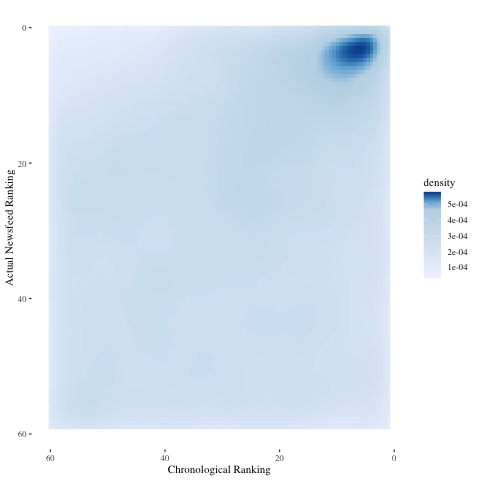
\includegraphics[width=1\linewidth]{Output/Graphs/Audit/Heatmaps/US NF chron rank by nf rank - smooth.jpg}   
        \caption{Chronology Heat Map}
        \label{fig:sub-first}
        \end{subfigure}
    \begin{subfigure}{.5\textwidth}
        \centering
        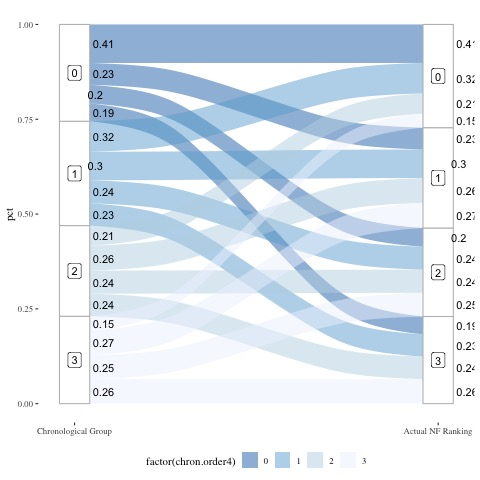
\includegraphics[width=1\linewidth]{Output/Graphs/Audit/Sankey flows/US NF chronology to actual.jpg}  
        \caption{Chronology Sankey (ALL!)}
        \label{fig:sub-second}
    \end{subfigure}

   \begin{subfigure}{.5\textwidth} 
        \centering
        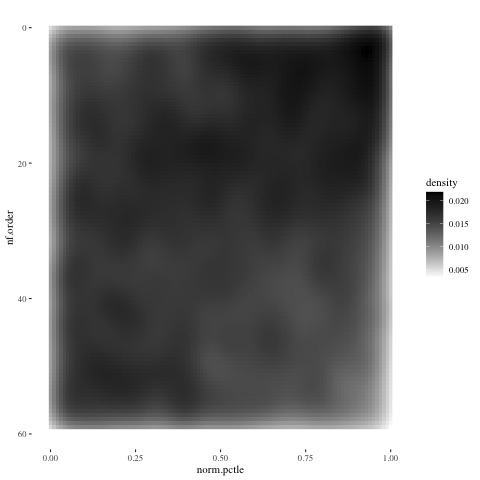
\includegraphics[width=1\linewidth]{Output/Graphs/Audit/Heatmaps/US NF norm pref rank by nf rank - smooth.jpg}  
        \caption{Preference Heat Map}
        \label{fig:sub-first}
        \end{subfigure}
    \begin{subfigure}{.5\textwidth}
        \centering
        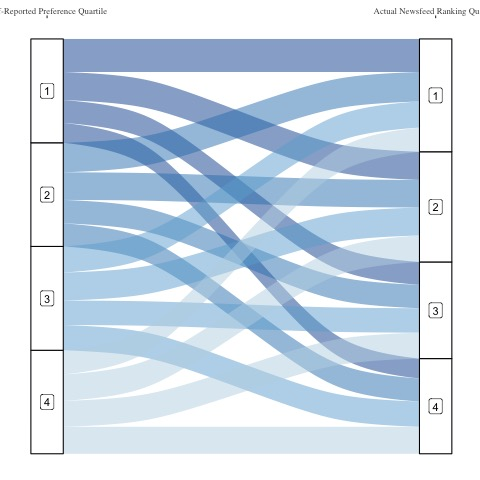
\includegraphics[width=1\linewidth]{Output/Graphs/Audit/Sankey flows/US NF norm quartile to actual.jpg}  
        \caption{Preference Sankey}
        \label{fig:sub-second}
    \end{subfigure}
    
\caption{NF Algorithm Does Algorithm Stuff}
\end{figure}



%%% NF Ingroup Posts %%%
\begin{figure}[ht]

    \begin{subfigure}{.5\textwidth} 
        \centering
        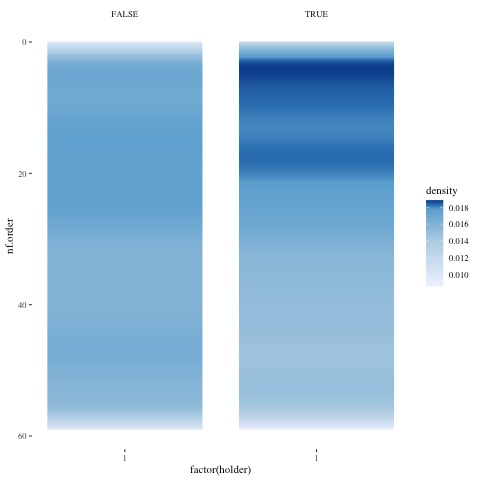
\includegraphics[width=1\linewidth]{Output/Graphs/Audit/Heatmaps/US NF nf rank by ingroup - smooth.jpg}  
        \caption{Two Single Heat Maps by Ingroup}
        \label{fig:sub-first}
        \end{subfigure}
    \begin{subfigure}{.5\textwidth}
        \centering
        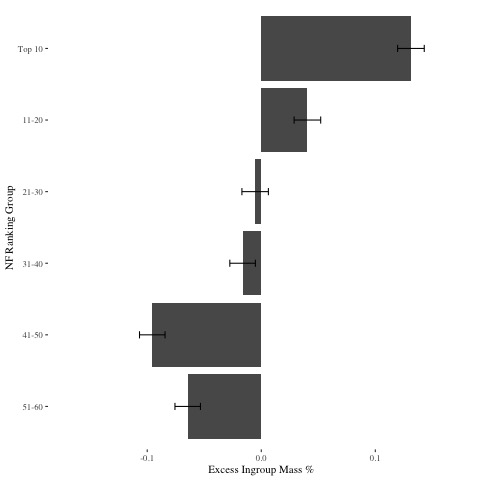
\includegraphics[width=.9\linewidth]{Output/Graphs/Audit/Excess Mass/US NF excess mass by ranking group.jpg}  
        \caption{Excess Mass by Ranking}
        \label{fig:sub-second}
    \end{subfigure}
\caption{NF Ingroup Posts Higher}
\end{figure}

%%% NF Ranking by preference %%%
\begin{figure}[ht]

    \begin{subfigure}{.5\textwidth} 
        \centering
            % include first image
        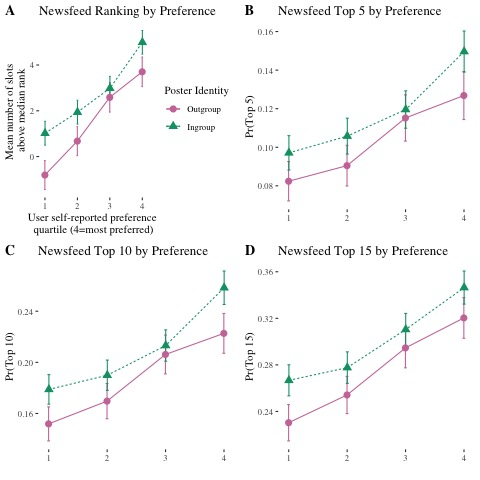
\includegraphics[width=1\linewidth]{Output/Graphs/Audit/Ranking line graphs/US NF all outcomes panel by norm preference by ingroup.jpg} 
        \caption{Something1}
        \label{fig:sub-first}
        \end{subfigure}
    \begin{subfigure}{.5\textwidth}
        \centering
        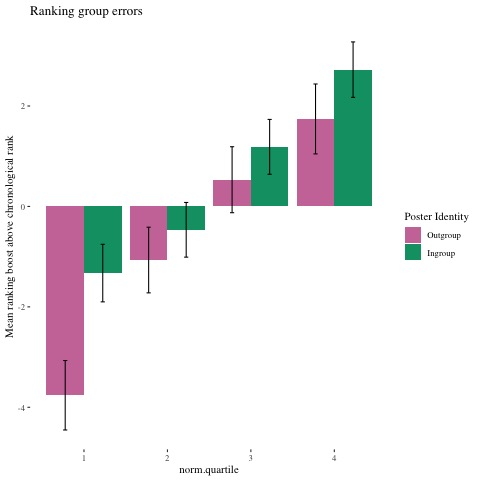
\includegraphics[width=1\linewidth]{Output/Graphs/Audit/Misranking relative to expectation/Chronological expectation/US NF by norm preference.jpg}  
        \caption{Something2}
        \label{fig:sub-second}
    \end{subfigure}
\caption{NF Beautiful Results}
\end{figure}

%%%%%%%%%%
%%% US: PYMK
%%%%%%%%%%

%%% NF Heatmap and Sankey: Chron vs Algorithm and Pref vs Algorithm %%%
\begin{figure}[ht]

    \begin{subfigure}{.5\textwidth} 
        \centering
        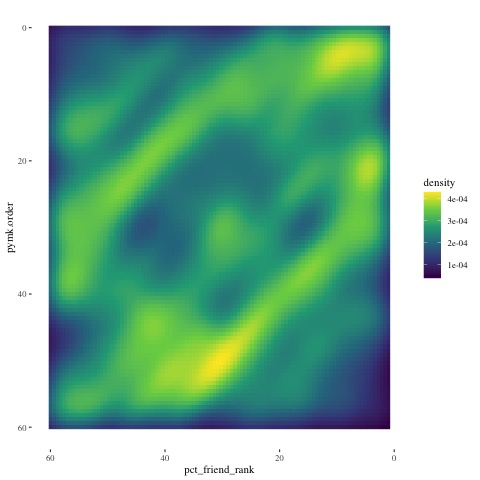
\includegraphics[width=1\linewidth]{Output/Graphs/Audit/Heatmaps/US PYMK pct friends by pymk rank - smooth.jpg}   
        \caption{Percent Friend Heat Map}
        \label{fig:sub-first}
        \end{subfigure}
    \begin{subfigure}{.5\textwidth}
        \centering
        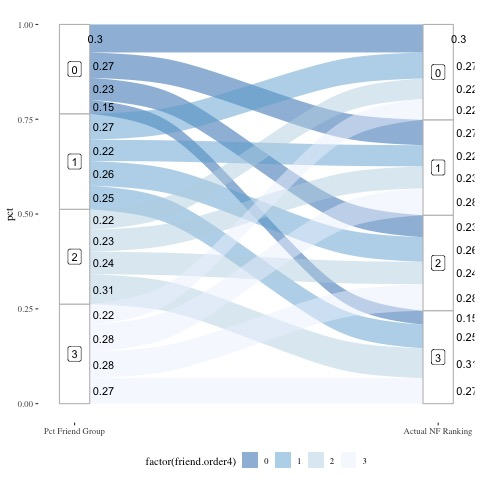
\includegraphics[width=1\linewidth]{Output/Graphs/Audit/Sankey flows/US PYMK pct friend to actual.jpg}  
        \caption{Percent Friend Sankey (ALL!)}
        \label{fig:sub-second}
    \end{subfigure}

   \begin{subfigure}{.5\textwidth} 
        \centering
        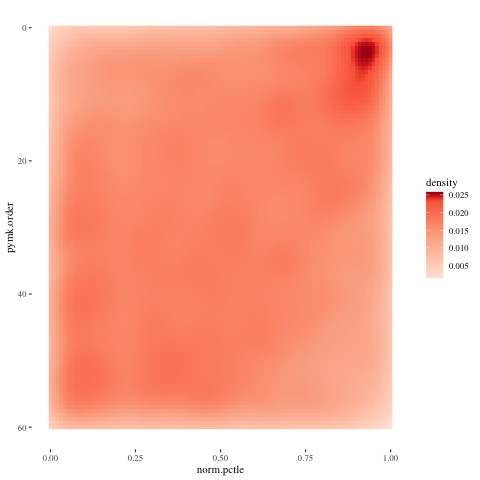
\includegraphics[width=1\linewidth]{Output/Graphs/Audit/Heatmaps/US PYMK norm pref rank by pymk rank - smooth.jpg}  
        \caption{Preference Heat Map}
        \label{fig:sub-first}
        \end{subfigure}
    \begin{subfigure}{.5\textwidth}
        \centering
        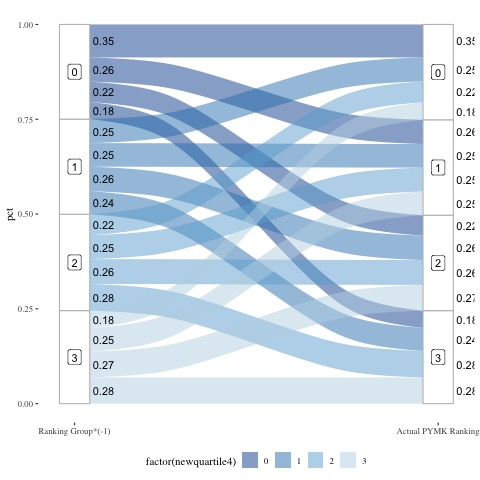
\includegraphics[width=1\linewidth]{Output/Graphs/Audit/Sankey flows/US PYMK norm quartile to actual.jpg}  
        \caption{Preference Sankey}
        \label{fig:sub-second}
    \end{subfigure}
    
\caption{PYMK Algorithm Does Algorithm Stuff}
\end{figure}


%%% PYMK Ingroup Posts %%%
\begin{figure}[ht]

    \begin{subfigure}{.5\textwidth} 
        \centering
        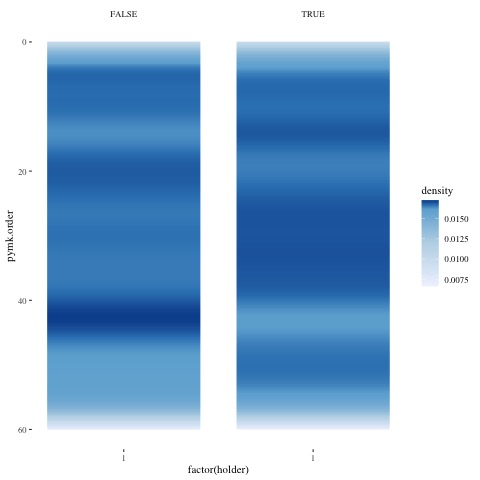
\includegraphics[width=1\linewidth]{Output/Graphs/Audit/Heatmaps/US PYMK pymk rank by ingroup - smooth.jpg}  
        \caption{Two Single Heat Maps by Ingroup}
        \label{fig:sub-first}
        \end{subfigure}
    \begin{subfigure}{.5\textwidth}
        \centering
        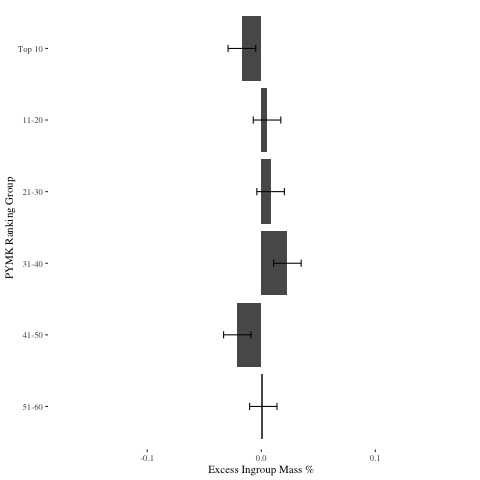
\includegraphics[width=.9\linewidth]{Output/Graphs/Audit/Excess Mass/US PYMK excess mass by ranking group.jpg}  
        \caption{Excess Mass by Ranking PUT ON SAME SCALE AS NF?}
        \label{fig:sub-second}
    \end{subfigure}
\caption{PYMK Ingroup Posts Not Higher}
\end{figure}

%%% NF Ranking by preference %%%
\begin{figure}[ht]

    \begin{subfigure}{.5\textwidth} 
        \centering
            % include first image
        \includegraphics[width=1\linewidth]{?} 
        \caption{Something1}
        \label{fig:sub-first}
        \end{subfigure}
    \begin{subfigure}{.5\textwidth}
        \centering
        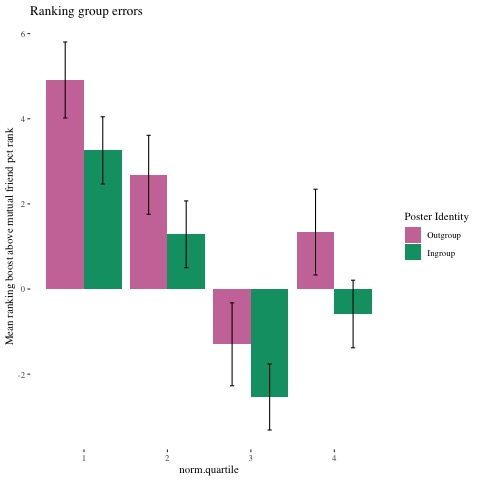
\includegraphics[width=1\linewidth]{Output/Graphs/Audit/Misranking relative to expectation/Mutual friends expectation/US PYMK by norm pref.jpg}  
        \caption{Something2}
        \label{fig:sub-second}
    \end{subfigure}
\caption{PYMK Results}
\end{figure}

%%%%%%%%%%
%%% US: AUTO
%%%%%%%%%%

\begin{figure}
    \begin{subfigure}{.5\textwidth} 
        \centering
        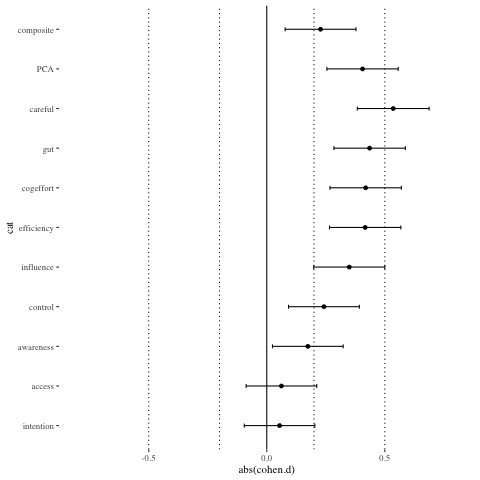
\includegraphics[width=1\linewidth]{Output/Graphs/Experiments/Automaticity/standardized effect sizes.jpg} 
        \caption{Standardized Effect Sizes)}
        \label{fig:sub-first}
    \end{subfigure}
    \begin{subfigure}{.5\textwidth} 
        \centering
        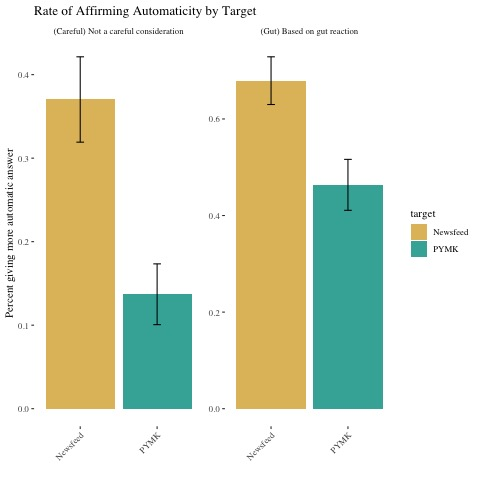
\includegraphics[width=1\linewidth]{Output/Graphs/Experiments/Automaticity/bar chart binary measures.jpg} 
        \caption{Just the binaries}
        \label{fig:sub-first}
    \end{subfigure}
    \begin{subfigure}{1\textwidth}
        \centering
        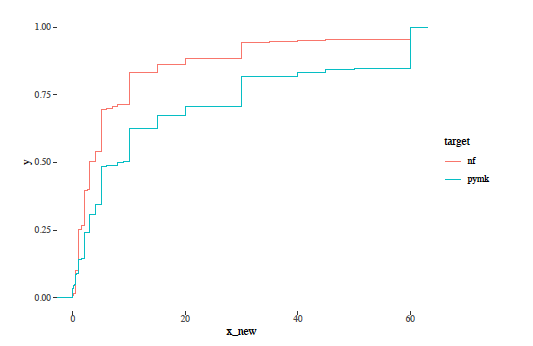
\includegraphics[width=.5\linewidth]{Output/Graphs/Experiments/Automaticity/speed cdf.png}  
        \caption{Speed (time to decide in seconds) CDF}
        \label{fig:sub-second}
    \end{subfigure}
\caption{Automaticity}
\end{figure}

%%%%%%%%%%
%%% US: Interactions
%%%%%%%%%%
\begin{figure}[!h]
    \centering
    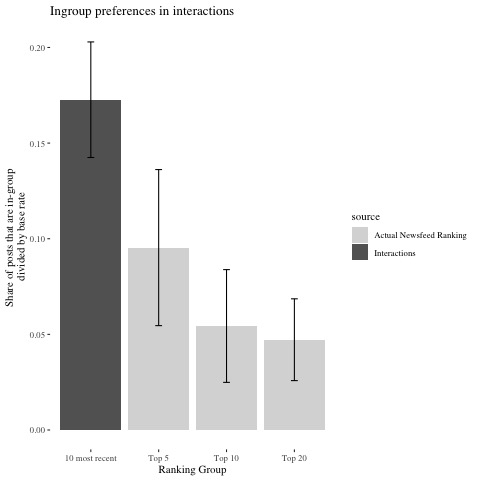
\includegraphics[width=1\linewidth]{Output/Graphs/Audit/Interactions/US preferences reactions and actual rankings above base rate.jpg}
    \caption{Beautiful Results}
    \label{fig:behavior}
\end{figure}


%%%%%%%%%% Appendix %%%%%%%%%%
\FloatBarrier
\clearpage
\appendix
\renewcommand\thefigure{\thesection.\arabic{figure}}
\renewcommand\thetable{\thesection.\arabic{table}}
\counterwithin{table}{section}

\section{Materials and Methods}\label{app:materials}

We collected data from XX participants over six sequential waves between March XX, 2020 and October XX, 2020. Over four waves we recruited 466 participants through the CDR (US); In a single wave we recruited 196 participants through HDSL (US); In a single wave we recruited 198 participants through CSBC (India). All waves share the same basic structure in which 1) participant privately completes a self-assessment, 2) RA guides each participant through the Newsfeed while recording information about each post and 3) RA guides participant through some additional data collection.

Data from each participant was collected in a single one-on-one Zoom session with an RA which lasted approximately one hour on average. After the data collection was completed, participants were sent a link to access their payment of \$20 (\$10 in India).

\subsection{Wave Overview}
\begin{itemize}
    \item Wave 1 - CDR, NF + PYMK, 242
    \item Wave 2 - HDSL, NF + PYMK, 196
    \item Wave 3 - India, NF + PYMK, 198
    \item Wave 4 - CDR, NF + Recent Activity, 54
    \item Wave 5 - CDR, NF (connectedness), 120
    \item Wave 6 - CDR, NF (about) + Recent Activity, 50
\end{itemize}

\subsection{Waves 1-3}

Waves 1-3 were nearly identical, each wave was on a different population. Because waves 1 and 2 were in the US, the group membership was based on perceived race, whereas wave 3 in India collected group membership based on perceived religion.

\subsubsection{Part I: Subject Categorization} After joining a Zoom call with an RA, subjects are asked to fill out a Qualtrics survey. In the survey, subjects are asked to describe their demographics and Facebook usage. As a main variable in our study, the assessment of the ingroup is paramount. US subjects are shown the seven race and ethnicity categories used in the US Census and are given the option to check as many boxes as they like. Indian subjects are asked to report their religion.

While the subject fills out the survey, the RA makes her best assessment of the subject’s ingroup (race in the US; religion in India), using up to two categories. Neither the subject nor the RA is aware of the assessment that the other has made. This protocol has the advantage of allowing us to observe how much alignment there is between how subjects self-identify and how they are perceived.

\subsubsection{Part II: Newsfeed} Users open their Facebook account and share their screen with the RA. Then, scrolling sequentially through each post in the Newsfeed, the subject answers exactly one question about each post: “There are more posts than Facebook can possibly show you. How would you rate this post on a scale from 1-7 where 1 means ‘can skip’ and 7 means ‘definitely want to see’.” In addition to recording the explicit preference, the RA assesses and records the perceived race of the poster of the content as well some other details of the post such as how long ago it was posted and whether it was posted to a group. The exact data being recorded by the RA are unknown to the subject. This continues for the first 60 non-sponsored posts.

\subsubsection{Part III: People You May Know} Subjects then navigate to the Facebook recommender for new friends, entitled “People You May Know” (PYMK). The procedure for this section is similar to that in Part II. The subject scrolls down the list and for each recommended user the subject answers one question: “How familiar are you with this person on a scale from 1-7?” In addition to recording the familiarity, the RA assesses and records the perceived race of the recommended user as well as the number of mutual friends. This continues for 60 recommendations.

\subsection{Wave 4}

Wave 4 differed slightly from the waves before it. Parts I and II were identical, but for part III instead of scrolling through the PYMK recommendation, particpants navigated to and scrolled through their 'recent activity' as follows.

\subsubsection{Part I: Subject Categorization} Identical to waves 1-3.

\subsubsection{Part II: Newsfeed} Identical to waves 1-3.

\subsubsection{Part III: Recent Activity} Subjects then navigate to the Facebook activity log, which is sorted in reverse chronological order. The RA instructs the participant to scroll down until identifying the first post with a reaction or comment. Then records perceived race and gender for the identified post. This process repeats for the 10 most recent comments/reactions to posts. As with NF data collection, if the race or gender of a user is not discernible from the post, the RA records the name in a separate list, and comes back to the list after collecting all 10 posts.

\subsection{Wave 5}

Wave 5 sought to collect richer data on the relationship between the participant and the author behind each Newsfeed post. There was no Part III in this wave.

\subsubsection{Part I: Subject Categorization} Identical to waves 1-4.

\subsubsection{Part II: Newsfeed} Users open their Facebook account and share their screen with the RA. Then, scrolling sequentially through each post in the Newsfeed, the subject answers exactly \textit{three} questions about each post: 
\begin{enumerate}
    \item “There are more posts than Facebook can possibly show you. How would you rate this post on a scale from 1-7 where 1 means ‘can skip’ and 7 means ‘definitely want to see’.” 
    \item How well do you know the person who posted this content? (1-7)
    \item How do you know this person? [Family, Friend, Acquaintance, Don’t know personally]
\end{enumerate}

In addition to recording the explicit preference, the RA assesses and records the perceived race of the poster of the content as well some other details of the post such as how long ago it was posted and whether it was posted to a group. The exact data being recorded by the RA are unknown to the subject. This continues for the first 60 non-sponsored posts.

\subsection{Wave 6}

Finally, Wave 6 sought to elicit participant perceptions on the purpose of the study 

\subsubsection{Part I: Subject Categorization} Identical to waves 1-5.

\subsubsection{Part II: Newsfeed}  Identical to wave 5.

\subsubsection{Part III: Recent Activity} Almost identical to wave 4, collecting 30 recent activity items instead of 10.

\subsubsection{Part IV: Study Purpose} RA asks the participant "What do you think this study is about?" and transcribes the answer as close to verbatim as possible.

\section{Additional Tables and Figures}\label{app:tab_fig}

%%% CDF US NF Preferences by Ingroup %%% 
\begin{figure}[!h]
    \centering
    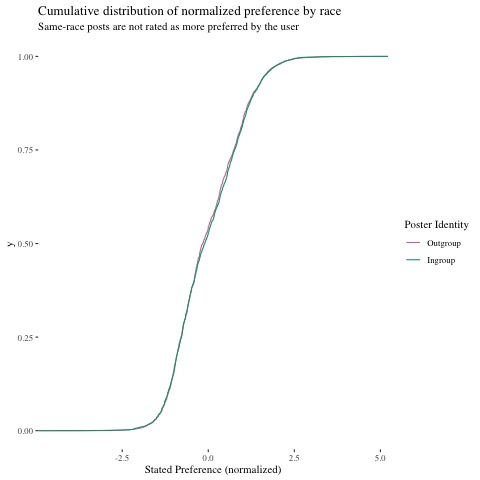
\includegraphics[scale=.8]{Output/Graphs/Audit/Stated preferences/US NF cdf norm preferences by ingroup.jpg}
    \caption{CDF}
    \label{fig:prefcdf}
\end{figure}


\section{India Results}\label{app:india}

\end{document}
